%
%

%%-----------------------------------------------------
%%-----------------------------------------------------
\section{Tres son multitud...}

%%-----------------------------------------------------
\begin{frame}
\frametitle{Los ataques ``man in the middle''}

\begin{columns}[T]
\begin{column}{.48\textwidth}
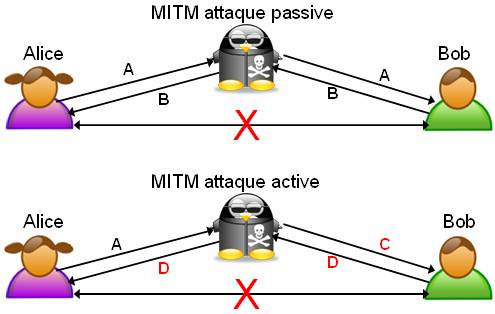
\includegraphics[width=6.5cm]{figs/man-in-the-middle}


\end{column}%
\hfill%
\begin{column}{.48\textwidth}
{\Large
\begin{itemize}
\item Monitorizar o alterar una comunicación.
\item Trivial en HTTP (texto claro).
\item HTTPS (TLS/SSL): \\
  Cifrado y certificados para evitarlo.
\end{itemize}
}
\end{column}%
\end{columns}
\vspace{1cm}
\begin{flushright}
{\footnotesize
Imagen ``Man in the Middle'', by Martial Régereau, CC by-sa 3.0 \\
\url{http://commons.wikimedia.org/wiki/File:Attaque_Man_In_The_Middle.jpg} 
}
\end{flushright}

\end{frame}

%%-----------------------------------------------------
\begin{frame}
\frametitle{Lenovo, Superfish y Komodia}

{\large
\begin{itemize}
\item Lenovo instala Superfish en varios modelos (octubre-diciembre 2014)
\item Se descubre que Superfish realiza ataque \\
  ``man in the middle'' para inyectar publicidad \\
\item Superfish instala un certificado de CA raíz, \\
  y establece un proxy para HTTP/HTTPS \\
\item Tecnología de Komodia, se usa en muchos sistemas (redes de empresas, software de control parental, etc.)
\item Al menos en algunos de ellos se han demostrado ataques ``man in the middle'' por terceras partes.
\end{itemize}
}

\begin{flushright}
{\footnotesize
\url{http://www.forbes.com/sites/thomasbrewster/2015/02/19/superfish-need-to-know/} \\
\url{http://arstechnica.com/security/2015/02/ssl-hijacker-behind-superfish-debacle-imperils-big-number-of-users/} \\
}
\end{flushright}
\end{frame}

%%-----------------------------------------------------
\begin{frame}
\frametitle{¿Cómo actúa Superfish en los Lenovo?}

{\Large
\begin{itemize}
\item Configura proxy para comunicación del navegador.
\item Instala un certificado de CA raíz propia.
\item Conexiones HTTPS ``capturadas'' por proxy.
\item De navegador a proxy, SSL con certificado firmado por la propia CA.
\item De proxy a sitio, SSL con certificado real.
\item Proxy: toda la comunicación en claro.
\item Certificados generados al vuelo: \\
  necesaria la clave privada de la nueva CA. \\
\item Resumen: terceros pueden leer conexiones HTTPS.
\end{itemize}
}

\begin{flushright}
{\footnotesize
\url{https://nakedsecurity.sophos.com/2015/02/20/the-lenovo-superfish-controversy-what-you-need-to-know/} \\
\url{http://blog.erratasec.com/2015/02/exploiting-superfish-certificate.html} \\
}
\end{flushright}
\end{frame}
